\documentclass[conference]{IEEEtran}
\IEEEoverridecommandlockouts
% The preceding line is only needed to identify funding in the first footnote. If that is unneeded, please comment it out.
\usepackage{cite}
\usepackage{amsmath,amssymb,amsfonts}
\usepackage{algorithmic}
\usepackage{graphicx}
\usepackage{textcomp}
\usepackage{xcolor}
\def\BibTeX{{\rm B\kern-.05em{\sc i\kern-.025em b}\kern-.08em
    T\kern-.1667em\lower.7ex\hbox{E}\kern-.125emX}}
\begin{document}

\title{Gaussian Mixtures in Machine Learning\\

%{\footnotesize \textsuperscript{*}Note: Sub-titles are not captured in Xplore and
%should not be used}
%\thanks{Identify applicable funding agency here. If none, delete this.}
%}

\author{\IEEEauthorblockN{Miguel Antonio Rodriguez Delgado}
%\IEEEauthorblockA{\textit{dept. name of organization (of Aff.)} \\
%\textit{name of organization (of Aff.)}\\
Dortmund, Germany \\
miguel-antonio.rodriguez-delgado@stud.hshl.de}
%\and
%\IEEEauthorblockN{2\textsuperscript{nd} Given Name Surname}
%\IEEEauthorblockA{\textit{dept. name of organization (of Aff.)} \\
%\textit{name of organization (of Aff.)}\\
%City, Country \\
%email address or ORCID}
%\and
%\IEEEauthorblockN{3\textsuperscript{rd} Given Name Surname}
%\IEEEauthorblockA{\textit{dept. name of organization (of Aff.)} \\
%\textit{name of organization (of Aff.)}\\
%City, Country \\
%email address or ORCID}
%\and
%\IEEEauthorblockN{4\textsuperscript{th} Given Name Surname}
%\IEEEauthorblockA{\textit{dept. name of organization (of Aff.)} \\
%\textit{name of organization (of Aff.)}\\
%City, Country \\
%email address or ORCID}
%\and
%\IEEEauthorblockN{5\textsuperscript{th} Given Name Surname}
%\IEEEauthorblockA{\textit{dept. name of organization (of Aff.)} \\
%\textit{name of organization (of Aff.)}\\
%City, Country \\
%email address or ORCID}
%\and
%\IEEEauthorblockN{6\textsuperscript{th} Given Name Surname}
%\IEEEauthorblockA{\textit{dept. name of organization (of Aff.)} \\
%\textit{name of organization (of Aff.)}\\
%City, Country \\
%email address or ORCID}
}

\maketitle

\begin{abstract}

Gaussian or Normal models help us to represent most of the distribution of all aspects of the world, showing how they can spread regarding the possibility for it to happen. This Gaussian models can allow us to distinguish between different set of points in an image for example. But in certain cases a point can be part of different groups. In this case Gaussian Mixtures can allow us to represent patterns which have elements in common. Gaussian Mixtures can be used in different fields. For example, to generate cancer detection algorithms.

\end{abstract}

\begin{IEEEkeywords}
Gaussian Mixtures, Deep learning, Machine learning.
\end{IEEEkeywords}

\section{Introduction}

In recent years there have been an increasing interest in deep learning algorithms for clustering detection, And deep neural networks have improved in the field of supervised classification \cite{deepgaussian}. Some important examples of this are present in Face-book deep face software detection \cite{deepgaussian}, prediction of pancreatic \cite{convolutional} and liver \cite{liver} cancer, among others.

Since Gaussian Mixtures are based on a combination of Gaussian Normal models, it is important to understand what is a Gaussian Normal mode (section \ref{normal_modes}). Then Gaussian Mixtures will be discussed (Section \ref{gmixtures}) and finally some examples on how Gaussian Mixtures can be applied on different research areas.

In \cite{aproxinter} and \cite{deepgaussian} we find a description on how Gaussian mixtures work in a general way. In reference \cite{random} is described how deep learning algorithm can be represented as Gaussian mixtures. And in \cite{convolutional} and \cite{liver} we can find examples on how to use Gaussian Mixtures to detect and predict pancreatic and liver cancer.

\section{Gaussian Models} \label{normal_modes}

Most of the parameters related on classification can be represented thought Gaussian Models \cite{normal_dist}. An simple example of this is the height of the population. In Fig. 1 we can see a representation of this. If we start analysing the figure from left to right we will see that the amount of short people is small, since is not very frequent to find small people. As we move on towards the middle of the graph, the amount of people start increasing, showing that most of the population will be present in this central part of the table. A proof of this in the real world, is that most of the people that we interact with is going to be near this height. But as we keep moving more to the right side of the graph, it will decrease again. Here once again we can see that the amount of tall people in our surroundings is not very high. This distribution will give us the shape of a bell. An this bell shape will be present in any distribution that we want to analyse. 

\begin{figure}
	\label{fig:height}
	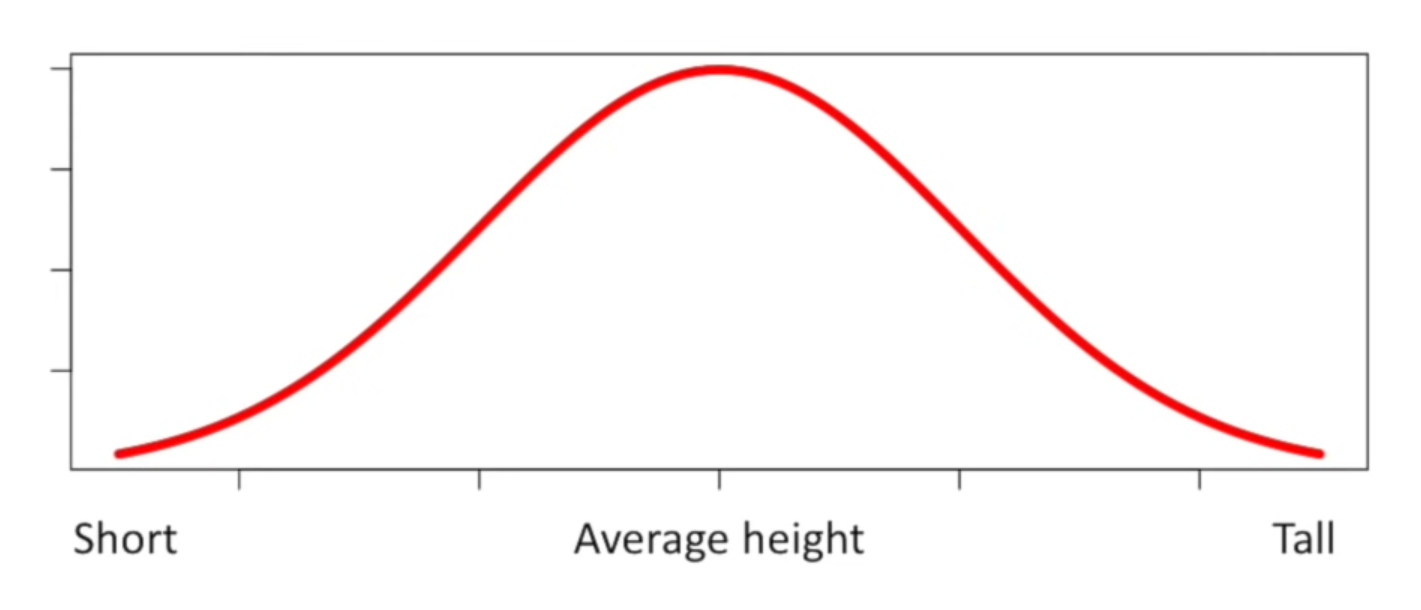
\includegraphics[scale=0.25]{imgs/height.png}
	\caption{Gaussian distribution of the population height. StatQuest with Josh Starmer. The Normal Distribution, Clearly Explained!!!. 2017.}
\end{figure}

Another example will be regarding the times on a race Fig. 2. The best racers will be on the left of the graph, that will represent the one or two racers that will pass the goal at first. Then while the race time increases there is more people that will arrive together, in this case not only one or two at the same time but maybe hundreds, and at the end of the graph we will find those that are less prepared and again at the end of the racers, it will pass only a few, normally just one or two.

\begin{figure}[h]
	\label{fig:race}
	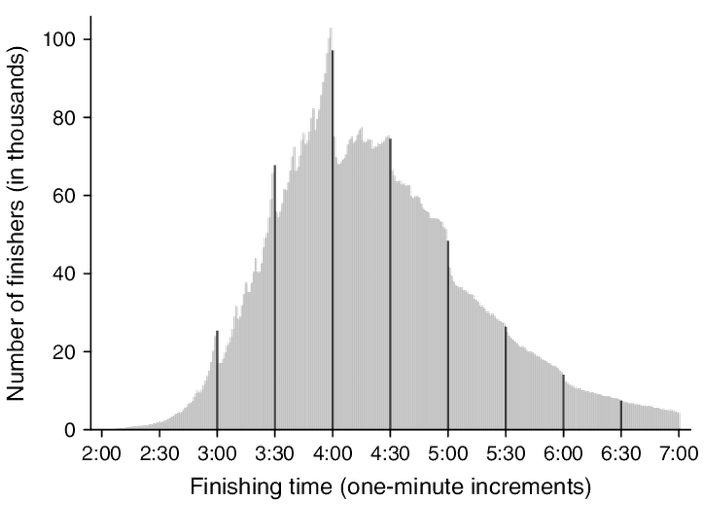
\includegraphics[scale=0.48]{imgs/race.png}
	\caption{Distribution of Marathon Finishing Times. Allen, Eric and Dechow, Patricia and Pope, Devin and Wu, George. (2016). Reference-Dependent Preferences: Evidence from Marathon Runners.}
\end{figure}

However this models will be capable to reproduce only single classification models.

\section{Gaussian Mixtures} \label{gmixtures}

Since most of the models that have to be analysed contain more that one single distribution, a mixture of these distributions is required.

Gaussian Mixture Models are used for clustering applications. Some examples of this are audio classification, document classification, segmentation for autonomous driving. In many cases the clustering process is well defined and using some clustering algorithms such as K-means clustering or Hierarchical clustering, but for the purpose of this seminar these algorithms will not be discussed.

Some data sets can be more complex and can have clusters that are intersecting with each other, so in these cases the we need an algorithm that will swap from Hard Clustering to Soft Clustering.

Hard clustering means that a point in the data set belongs only to one group, while in soft clustering a point can belong a determinate percentage to a different amount of groups.

Gaussian mixtures are based in normal distributions, that as we have seen in the previous section will tell us in which proportion a point belongs to a group.

\subsection{Clustering points}

In a Gaussian mixture a point can belong to two different groups. The way that the Gaussian mixture will assign a point to a cluster will depend on how far and how probable is that a point belongs to cluster and in which percentage it does. For example in Fig. 3 if we have a set of points and two Gaussian the points will belong to the yellow or the blue cluster, all the points that are inside the blue cluster, or in the left part of the graph belong to the blue Gaussian, the points that are inside the yellow cluster or in the left side of the graph belong to the yellow Gaussian, and the points that are between the two colors, will belong in a certain percentage to both of the clusters.


\begin{figure}[h]
	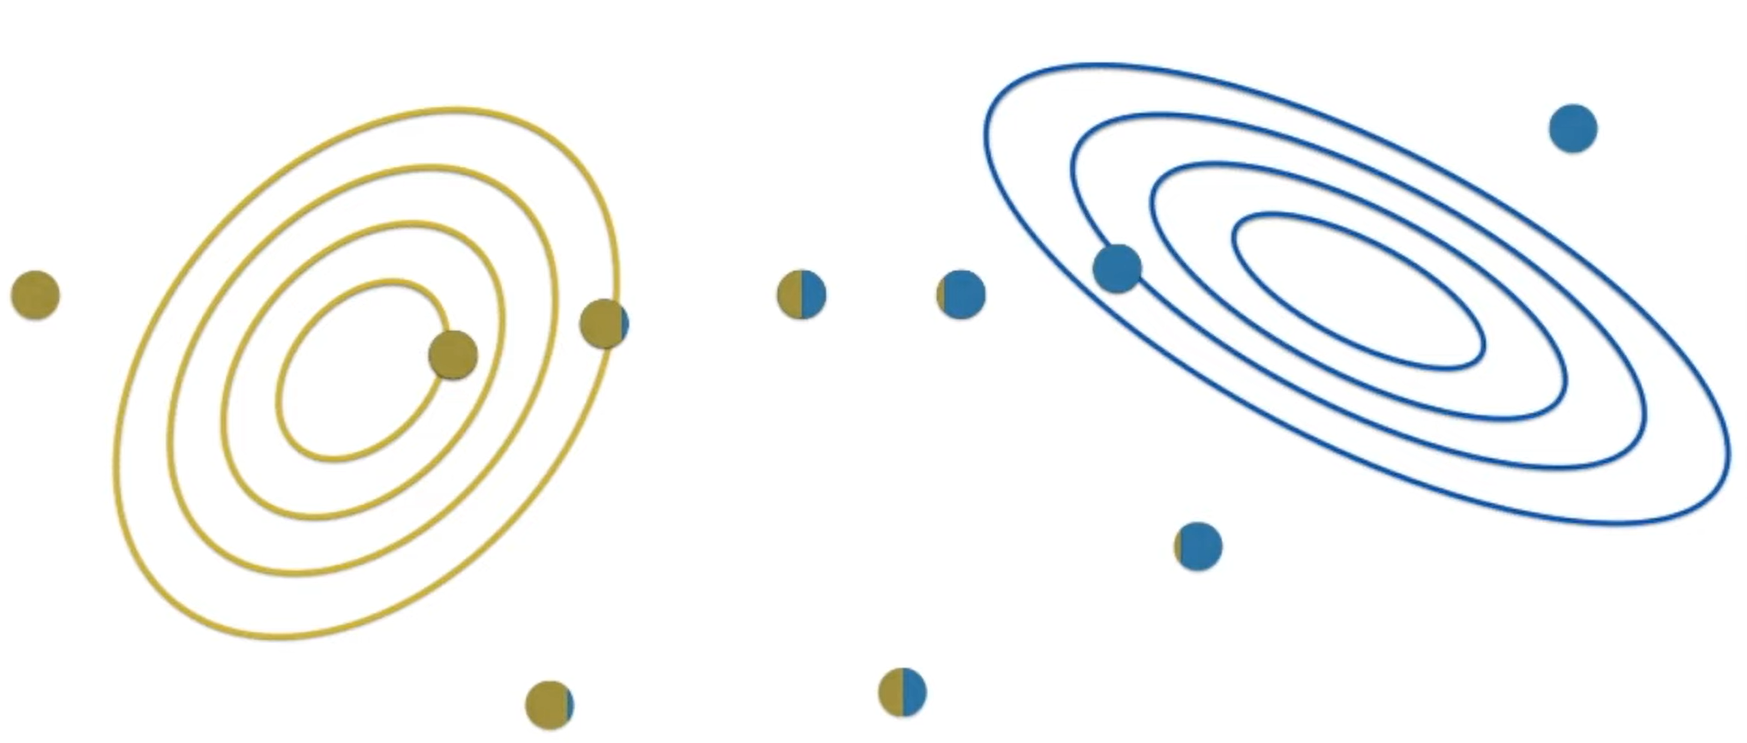
\includegraphics[scale=0.19]{imgs/gaussian1.png}
	\label{fig:gaussian}
	\caption{Colouring points. Luis Serrano. Gaussian Mixture Models. 2020}
\end{figure}

To define the percentage in which a point belongs to a group the Gaussian Normal model o the Gaussian distribution that we saw before will be use. For example, we can call the yellow cluster $f(x)$ and the blue cluster $g(x)$. Each one of this functions will represent a Normal distribution, the points that are nearest or under the center of the bell will belong to an area or a cluster and they will have a high percentage regarding to this group, and the ones that are far from the center or in the borders of the bell can still belong to the cluster but in a smaller percentage. 

In Fig. 4 we can see an example on how Normal distributions can be used to assign a different percentage value to different points. If we look at the points left to right, we will see that the first point has a biggest influence under the yellow Gaussian ($f(x)$) than under the blue Gaussian ($g(x)$). for this point the values assigned could be around 75\% of probability to belong to the yellow area and 25\% to belong to the blue area. The second point will probably have 50\% of probabilities to belong to both areas, and the third point could belong in a 95\% to the blue Gaussian and 5\% to the yellow one.

\subsection{Fitting a Gaussian}

To get a good fitting for a Gaussian we will have to take all the points that belong to a cluster and to get the center of this cluster. To do this we calculate the $x$-variance, the $y$-variance and the covariance to calculate the center of mass of the system. The formulas used for this are the next ones.

\begin{figure}[h]
	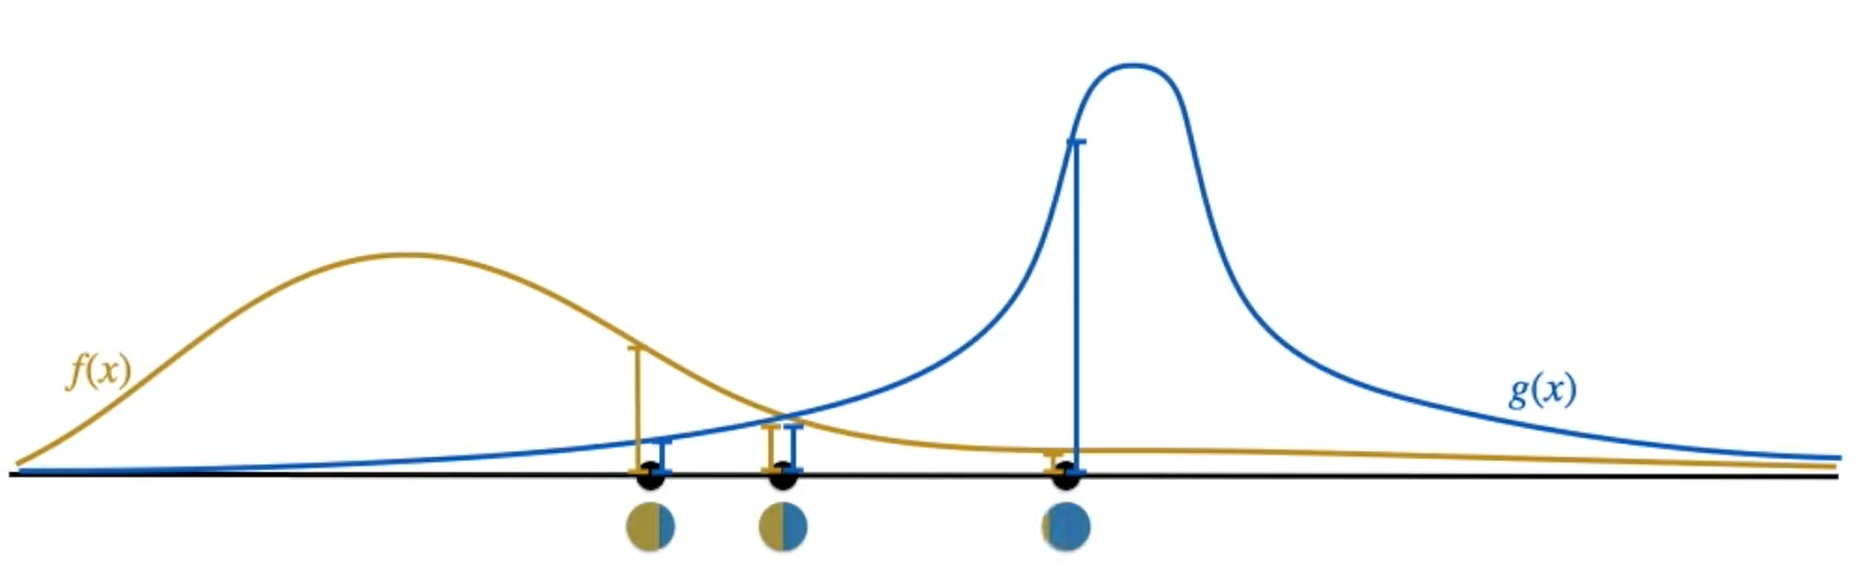
\includegraphics[scale=0.19]{imgs/gaussian2.png}
	\label{fig:gaussian2}
	\caption{Colouring points with normal distributions. Luis Serrano. Gaussian Mixture Models. 2020}
\end{figure}

There are other values that have to been taken into account to calculate the center of mass, for example the percentages that a point have in a cluster to give a better center result but for the purposes of this seminar, the mathematical formulas will not be discussed deeply.

\subsection{Gaussian Mixture Algorithm}

The Gaussian Mixture Algorithm is based in three main steps. starting random Gaussian models, fitting the points to the Gaussian models and recalculating the Gaussian models regarding the values that have been fitted on them.

For the first step the algorithm will not know where are the points located or how are they clustered. For this reason, the Gaussian models will start randomly. After this a loop containing the second and third part of the algorithm, this algorithm will run as many times as required, this will be until the algorithm is not converging.

Inside the loop, the algorithm will assign the point to a Gaussian using the fitting Gaussian method that we saw before. The points will be given a percentage value to belong to one or another Gaussian. After this, the the algorithm will recalculate the center of the Gaussian models with the information of the points that have been fitting to it. After this, with the new calculated Gaussian models, the algorithm will be given new percentages, and they will be assigned again to the respective Gaussian with the new values, and the center of the Gaussian will be calculated again. This process will continue while the algorithm is not converging.

An example of this process can be found on Fig 5. The first part is defining random Gaussians, then the points are coloured according how near they are to the respective Gaussian, then the Gaussians are recalculated, the points are coloured again, and this proces continues until the Gaussian Mixture converges.

\begin{figure}[h]
	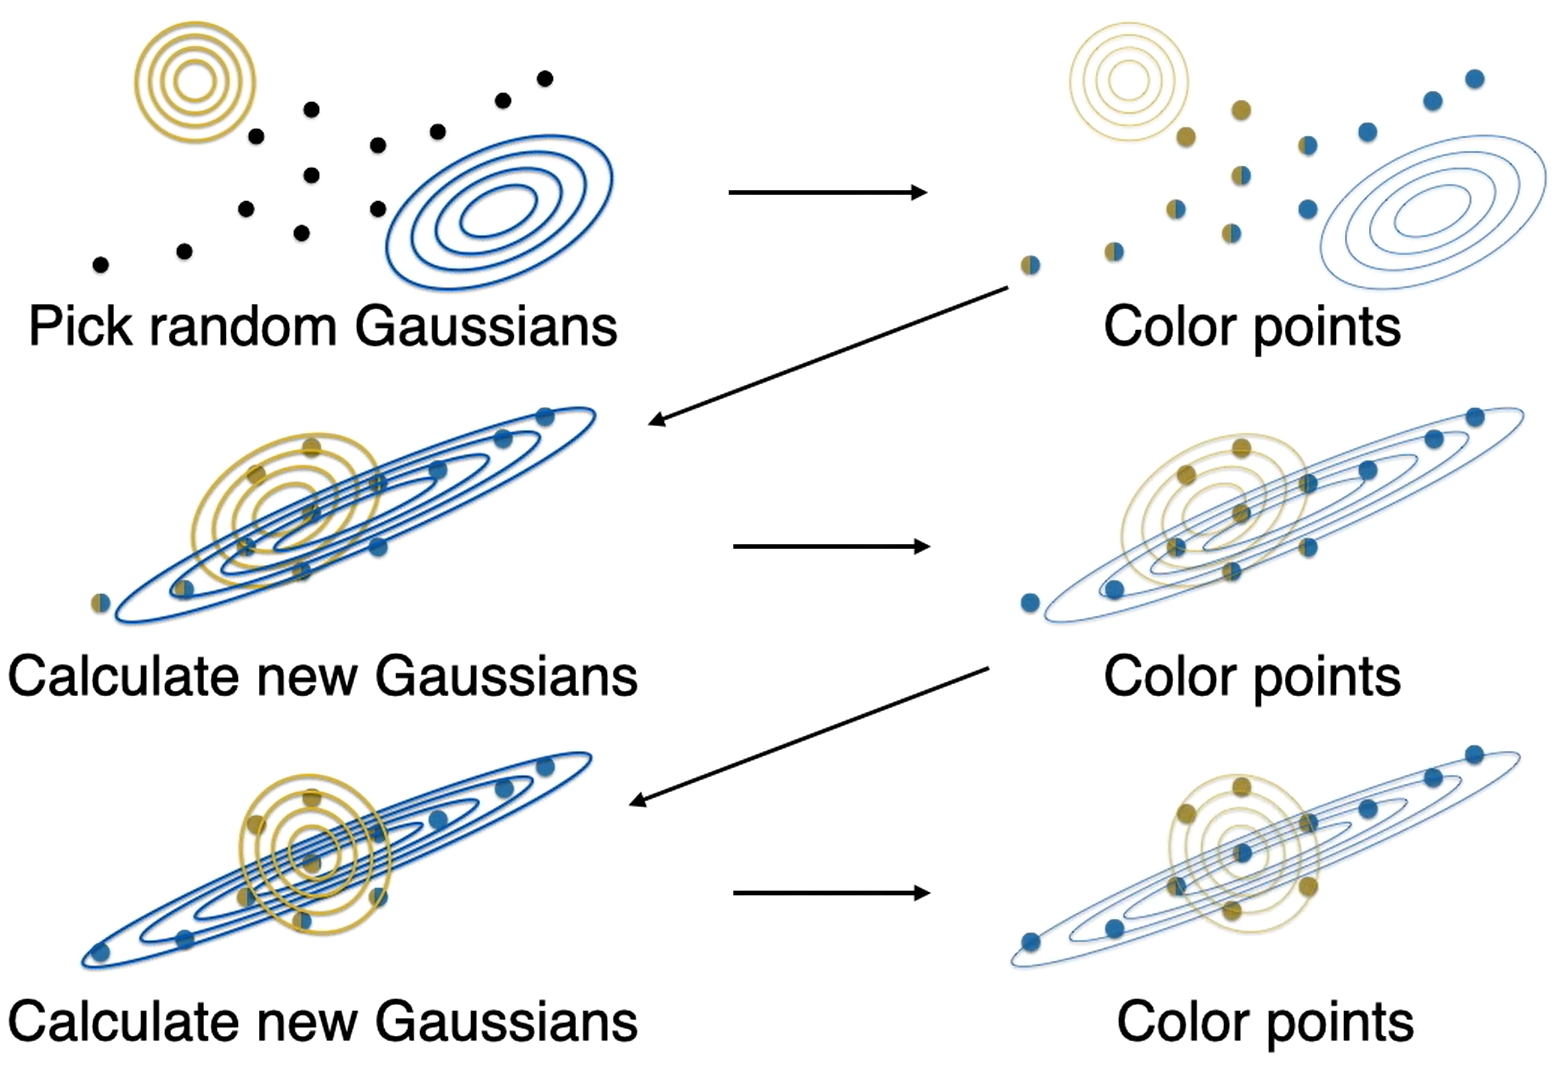
\includegraphics[scale=0.22]{imgs/gaussian3.png}
	\label{fig:gaussian}
	\caption{Gaussian Mixtures process. Luis Serrano. Gaussian Mixture Models. 2020}
\end{figure}

\section{Conclusion} 

The Gaussian Mixture is a soft clustering model that allows to gather members for the cluster based on the probabilities that the point belong to it. This method can be use to cluster data that is not well defined and that can be difficult to cluster with hard clustering methods.

%
%\begin{table}[htbp]
%\caption{Table Type Styles}
%\begin{center}
%\begin{tabular}{|c|c|c|c|}
%\hline
%\textbf{Table}&\multicolumn{3}{|c|}{\textbf{Table Column Head}} \\
%\cline{2-4} 
%\textbf{Head} & \textbf{\textit{Table column subhead}}& \textbf{\textit{Subhead}}& \textbf{\textit{Subhead}} \\
%\hline
%copy& More table copy$^{\mathrm{a}}$& &  \\
%\hline
%\multicolumn{4}{l}{$^{\mathrm{a}}$Sample of a Table footnote.}
%\end{tabular}
%\label{tab1}
%\end{center}
%\end{table}
%
%\begin{figure}[htbp]
%\centerline{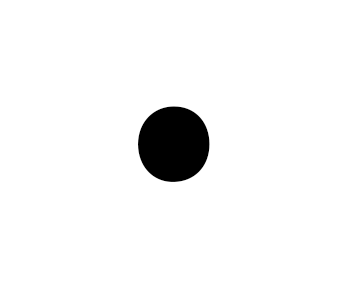
\includegraphics{fig1.png}}
%\caption{Example of a figure caption.}
%\label{fig}
%\end{figure}


\begin{thebibliography}{00}
\bibitem {random} 
Seddik, M.E.A., Louart, C., Tamaazousti, M., \& Couillet, R.. (2020). Random Matrix Theory Proves that Deep Learning Representations of GAN-data Behave as Gaussian Mixtures. <i>Proceedings of the 37th International Conference on Machine Learning</i>, in <i>Proceedings of Machine Learning Research</i> 119:8573-8582 Available from https://proceedings.mlr.press/v119/seddik20a.html.

\bibitem{convolutional}
Sekaran, K., Chandana, P., Krishna, N.M. et al. Deep learning convolutional neural network (CNN) With Gaussian mixture model for predicting pancreatic cancer. Multimed Tools Appl 79, 10233–10247 (2020). https://doi.org/10.1007/s11042-019-7419-5

\bibitem{deepgaussian}
Viroli, C., McLachlan, G.J. Deep Gaussian mixture models. Stat Comput 29, 43–51 (2019). https://doi.org/10.1007/s11222-017-9793-z

\bibitem{aproxinter}
Nalisnick, E.T., Hertel, L., \& Smyth, P. (2016). Approximate Inference for Deep Latent Gaussian Mixtures.

\bibitem{liver}
Amita Das, U. Rajendra Acharya, Soumya S. Panda, Sukanta Sabut,
Deep learning based liver cancer detection using watershed transform and Gaussian mixture model techniques,
Cognitive Systems Research,
Volume 54,
2019,
Pages 165-175,
ISSN 1389-0417,
https://doi.org/10.1016/j.cogsys.2018.12.009.
(https://www.sciencedirect.com/science/article/pii/S1389041718310143)

\bibitem{normal_dist}
The Normal Distribution, Clearly Explained!!! (2017, 9 oktober). YouTube. Geraadpleegd op 29 april 2022, van https://www.youtube.com/watch?v=rzFX5NWojp0

\bibitem{race}
Allen, Eric and Dechow, Patricia and Pope, Devin and Wu, George. (2016). Reference-Dependent Preferences: Evidence from Marathon Runners. Management Science. 63. 10.1287/mnsc.2015.2417. 

\bibitem{mixture_models}
Gaussian Mixture Models. (2020, 28 december). YouTube. Geraadpleegd op 29 april 2022, van https://www.youtube.com/watch?v=q71Niz856KE

\end{thebibliography}

\end{document}
